
Data set elements can be mapped to specific visual features of tag clouds - these features  relate almost entirely to font characteristics. Phrase or keyword emphasis in tag clouds are taken from typographical techniques, the ancient art of arranging type. Typography can be applied with a long and varied list of principles such as those outlined in the seminal typography manual ``The elements of typographical style'' \citep{bringhurst01}. There are several typographic ways of creating emphasis in text such as size, colour, typeface, weight and italics, and these may all be employed within tag clouds to draw attention to keywords or phrases of importance. Visual properties of tag clouds that may be manipulated for effect include (see Fig. \ref{fig:mapping} for an example of data mapped to some of the following properties);

\begin{enumerate}
   	\item Layout
   	\item Text size
   	\item Background colour contrasts (hue, saturation, value)
    	\item Text colour contrasts (hue, saturation, value) 
    	\item Background colour transparency
    	\item Text colour transparency 
    	\item Typeface family (e.g. Serif vs Sans-serif or Arial, Times New Roman) 
    	\item Typeface style bold (bold, normal)
    	\item Typeface style italics ( italics, normal) 
    	\item Typeface style all capitals (all capitals, mixed case)
    	\item Typeface style underline (underline, normal) 
\end{enumerate}

\begin{figure}[h!]
	\centering
	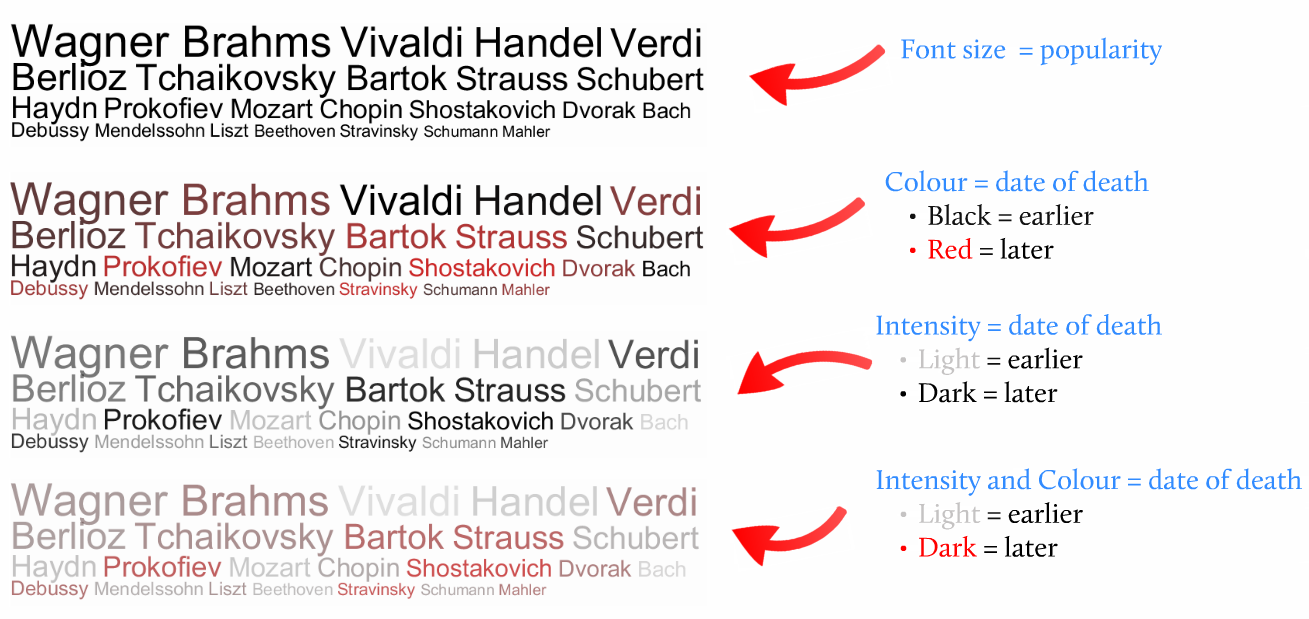
\includegraphics[scale=0.45]{mapping.png}
	\caption{\emph{Popularity Ranking of Composers:} mapping (synthetic) data to tag cloud visual properties.}
	\label{fig:mapping}
\end{figure}

`Visual Variables', as introduced by \citet{bertin83} in the `Semiology of Graphics', are a specified set of symbols that can be applied to data in order to translate information. This process of mapping data to visual properties is called `visual mapping'. These visual variables were defined as position, size, shape, value, colour (hue), orientation, and texture. Choosing a particular variable to map to data depends on an analysis of the characteristics of the variable. Each variable's characteristics are defined from the following list:

\begin{itemize}
	\item Selective: If a data point can easily be selected from the other marks.
	\item Associative: If multiple data points can be grouped across changes in other variables.
 	\item Quantitative: If differences in underlying data can interpreted numerically.
 	\item Order: If data points in a variable can be interpreted in an order.
	\item Length: How many values a variable can meaningfully contain.
\end{itemize}

\subsection{Size} 

Text size manipulation can be a very effective way of creating emphasis, providing the size increase is large enough (see Fig. \ref{fig:fontseries} for a depiction of the traditional size variation in a font series). Empirical research on tag cloud visual properties has identified size as having a significant effect of user perception \citep[such as][]{lohmann09, bateman08, halvey07}. According to Bertin, the size visual variable is selective, associative, and quantitative \citep{bertin83}. However, care must be taken when using size quantitatively, as changes in size from volume or area are difficult to interpret \citep{carpendale03}. This is an important point as tag cloud data mapping in the software engineering domain will often be of a numerical nature. With regards to length (the range of values possible to display in a variable) it is thought that if data points are adjacent then size variations from approximately 40 to 50 might be used. If placed separately in the display (such as in tag clouds), then the size variations might be limited to something in the order of approximately 5. Finally, research has indicated slower reading performance when font sizes are less than 12pts and that it is unwise to display less than a 9pt font on a web page \citep[pg 107, chap 11:8][]{usability06}. To summarise, size manipulation can be a very effective way of emphasising keyword or phrase importance within a tag cloud, provided careful consideration is given to size variations. 

\begin{figure}[h!]
  \centering
  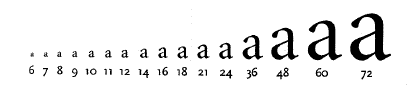
\includegraphics{typesize.png}
  \caption{Traditional Font Size Series}
  \label{fig:fontseries}
\end{figure}

\subsection{Background Colour}

\citet{preston10} investigated the effectiveness of typographical emphasis techniques (such as colour, bold and italics) on computer presentation software. They found that chromatic emphasis techniques - those using colour - generally elicited significantly faster response times identifying emphasised text than achromatic techniques such as bold and italic, provided a suitable colour contrast was given. Examples of appropriate colour contrasts given were red, green or blue on a white background; red, green, yellow or blue on a black background; or red, yellow and green on a dark blue background. Examples of inappropriate colour contrast were blue on a dark blue background or yellow on a white background. These results indicate careful consideration of text colour against background must be given during colour selection of visual mappings within a tag cloud.

It is possible to manipulate background colour on an individual tag. This could have two possible benefits 1) it may be an effective way of grouping together multiple keywords or phrases and 2) because the area of the background behind the tag is greater than area of the font text itself, mapping the colour to the background behind the tag may have a greater effect on user perception than mapping the colour to the text. See Fig. \ref{fig:background} for examples of text and foreground colour.

\begin{figure}[h!]
  \centering
  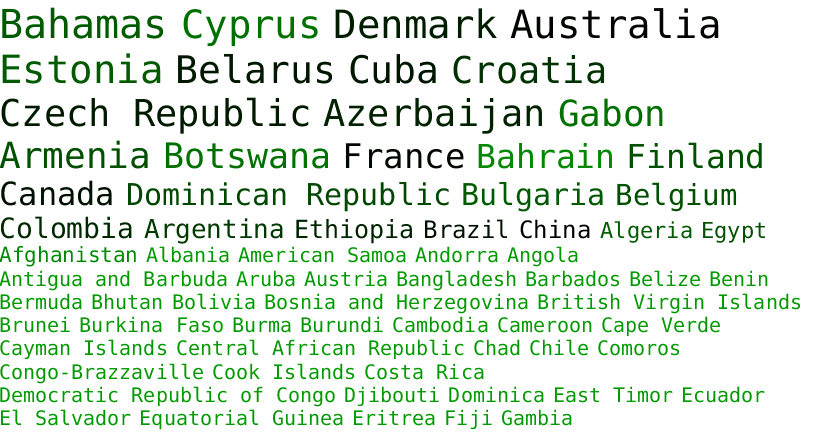
\includegraphics[scale=0.60]{foregroundex.png}
  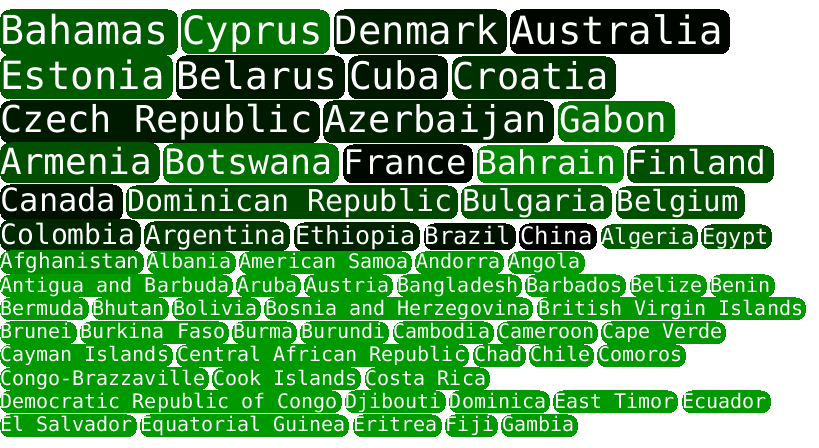
\includegraphics[scale=0.60]{backgroundex.png}
  \caption{Official and population based Olympic medal rankings - shown in font colour and background colour.}
  \label{fig:background}
\end{figure}

\subsection{Text Colour (Hue, Saturation and Value)}

\citet{bateman08} found that colour intensity (saturation) had a relatively good influence on user perception (although not as strong and font size or weight). However, they found the colour hue in text to have an unreliable influence and were unable to establish to what degree and which colours were more likely to draw the attention of a viewer.  Value is said by Bertin to have properties selective, associative and ordering \citep{bertin83}, whereas colour hue has only selective and associative properties and cannot be perceived by a viewer in an ordered fashion. Value may be considered to be quantitative also in that lighter value colours are percieved to be related to smaller numbers and darker colour values of higher numbers, but actual quantitative comparison is difficult (for example perceiving one shade of colour as being 3 times darker than another shade). The number of differing values (length characteristic) which may be easily perceived by a viewer for both hue and value is thought to be less than 7 \citep{carpendale03}. These results indicate that colour value or saturation may be more effective data mapping variables than colour hue within a tag cloud.

\subsection{Font Style (Bold, Italic, Underline and Capitals)}   

\citet{bateman08}'s exploration of the effects of various properties and characteristics of text in tag clouds found that weight (bold style) had a consistently strong influence on user perception. Experiments by \citet{preston10} found bold text performed well with black text on a white background but not with white text on black.  \citet{preston10} found capitals to be the most effective of the achromatic emphasis techniques although all four techniques did not perform as well as the chromatic techniques (use of colour).  Underline and italic emphasis techniques were consistently the least effective means of emphasising text. Font styles or typography in general were not included in Bertin's visual variables \citet{bertin83}. However, the number of values that these typography styles may show is very small (Bertin's variable length) - just two differing values. Although font styles bold or underline appear to be more effective at text emphasis than italic or underline, the number of differing values they may show is so small they are likely not worth including as a data mapping variable in a tag cloud.

\subsection{Font Family}   

Typographical characteristics such as font family were not mentioned by \citet{bertin83}. However, the shape visual variable, which is the most closely related variable mentioned, is not perceived as an especially effective variable. According to \citet{carpendale03}, shape may be selective and associative, providing there are minimal data points or minimal shape variations. Wit the number of shape variations required in mapping font family to software engineering or other general data, it does not seem that font family would be an effective mapping too. Additionally, there is the possibility that manipulation of font family may alter user perception of other font styles used as a mapping variable, such as bold or italic. Finally, research shows that reading speed is best when users are presented with familiar fonts such as Times New Roman, Arial or Helvetica  \citep[pg 106, chap 11:7][]{usability06}. To summarise, usage of font family as a data mapping variable within a tag cloud might not be optimal, and a familiar font such as Arial is preferable for reading accuracy.

\subsection{Hierarchical Information} 
Visual variables which have the characteristic of `order' may be used to show hierarchies among data. These variables are position, size and colour value. These variables combined may serve to either strengthen the user perception of one data variable or show the difference in hierarchies of multiple data variables \citep{deeb12}. There is some evidence to suggest two levels of hierarchy is preferred over three when varying typographical visual variables \citep{deeb12}.


%Order of visual influence according to \citet{bateman08}:
%\begin{itemize}
%	\item Font size
%	\item Typeface style (bold) - can override font size in some situations
 %	\item Colour saturation (text)
 %	\item Colour (text) - influence unreliable
%\end{itemize}


%Order of visual influence according to \citet{preston10}:
%\begin{itemize}
%	\item Colour (text, background) - given appropriate contrast 
%	\item Typeface style (bold) - on a white background
% 	\item Typeface style (all capitals)
 %	\item Typeface style (italic)
 %	\item Typeface style (underline)
%\end{itemize}



% ------------------------------------------------------------------------

%%% Local Variables: 
%%% mode: latex
%%% TeX-master: "../thesis"
%%% End: 
